\section{Test Plan}

The following steps have been made to test the proper functioning of every part of the Linear Interpolator:

\begin{enumerate}
    \item \textbf{Ripple Carry Adder}, \textbf{D Flip Flop} and \textbf{Counter} have been tested independently, using separate test bench.
    \item The \textbf{Combinational Network} has been tested through comparison with specific values previously decided.
    \item The same values are been used to test the total \textbf{Linear Interpolator}.
    \item Two \textbf{scripts} have been made to test the total circuit with \textbf{signals dynamically generated}.
\end{enumerate}

\subsection{Basic Circuits Test}

The \textbf{Ripple Carry Adder} has been tested by choosing specific values for the input, and checking that the values of outputs represent the right sum and carry out.

\begin{figure}[H]
    \centering
    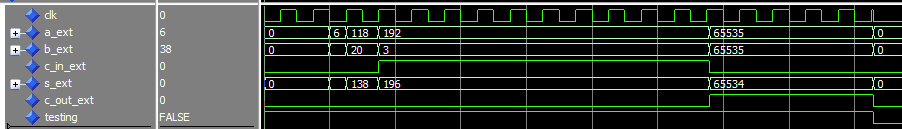
\includegraphics[width=1\textwidth]{img/Chapter4/rca.png}
    \caption{Ripple Carry Adder Test}
    \label{fig:RCATest}
\end{figure}

For the \textbf{D Flip Flop} has been tested the ability to save and keep stable the values received in input. Moreover, has been tested the proper functioning of enabler port.

\begin{figure}[H]
    \centering
    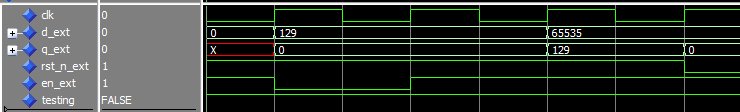
\includegraphics[width=1\textwidth]{img/Chapter4/dff.png}
    \caption{D Flip Flop Test}
    \label{fig:DFFTest}
\end{figure}

For the \textbf{counter}, the output was tested as the various clock cycles passed:

\begin{figure}[H]
    \centering
    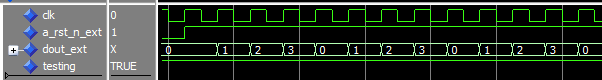
\includegraphics[width=1\textwidth]{img/Chapter4/counter.png}
    \caption{CounterTest}
    \label{fig:CounterTest}
\end{figure}

\subsection{Combinational Network Test}

In order to test the proper functioning of \textbf{Combinational Network}, an Excel file has been made, shown in the following figure: 

\begin{figure}[H]
    \centering
    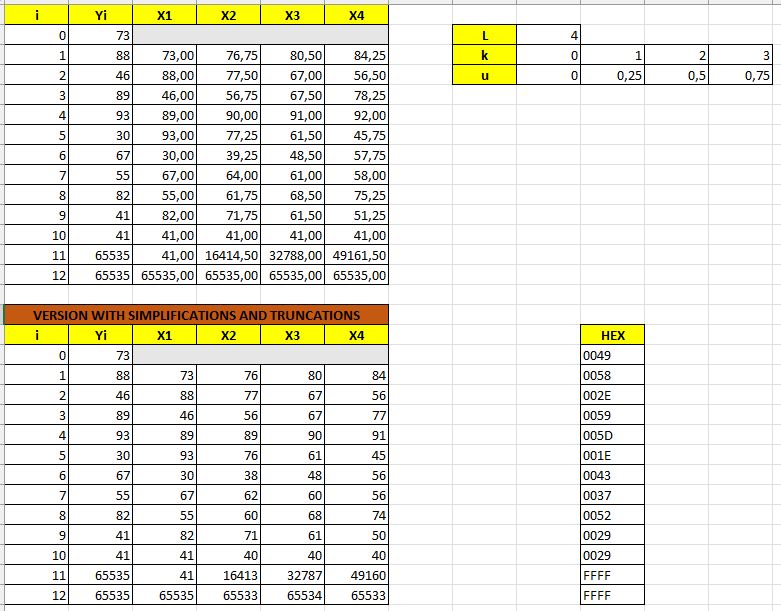
\includegraphics[width=0.8\textwidth]{img/Chapter4/Excel.png}
    \caption{Test Plan for Combinational Network}
    \label{fig:CNExcel1}
\end{figure}

In this file a series of values have been dynamically generated, and they are used to compute the linear interpolation with and without simplification (shift for division, etc...).

After that, some of this values are used to create the stimuli for the Combinational Network, in a test bench specifically created. The correctness of the results has been verified through a visual analysis. The ModelSim simulation obtained is the following:

\begin{figure}[H]
    \centering
    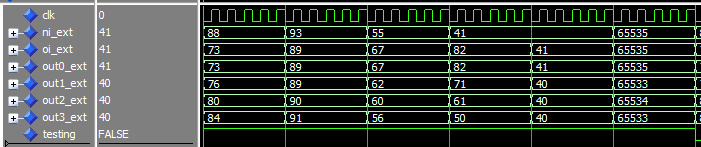
\includegraphics[width=1\textwidth]{img/Chapter4/CI.png}
    \caption{Combinational Network Test}
    \label{fig:CNTest}
\end{figure}

Moreover, in the Excel file there are both approximated and effective interpolated signals, so it is possible to compute the mean error, as shown below:

\begin{figure}[H]
    \centering
    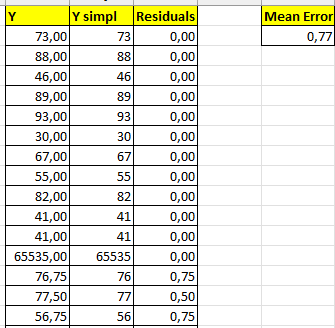
\includegraphics[width=0.4\textwidth]{img/Chapter4/Error.png}
    \caption{Mean Error caused by the simplifications}
    \label{fig:CNExcel2}
\end{figure}

It's clear that in this case the mean error is below one; This confirms the hypothesis that the error caused by the approximation is acceptable.

\subsection{Linear Interpolator Test}

As said before, the values obtained in the previous Excel file (Figure \ref{fig:CNExcel1}), has been used even in the \textbf{Linear Interpolator} test. The following figure represents the stimuli used in the test bench:

\begin{figure}[H]
    \centering
    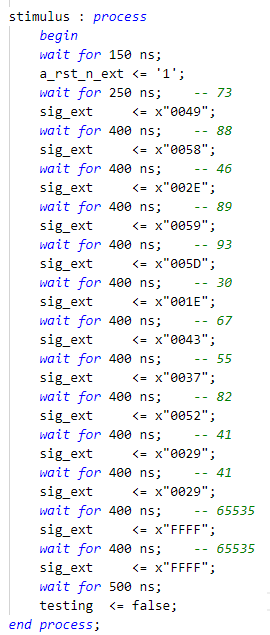
\includegraphics[width=0.3\textwidth]{img/Chapter4/Stimuli_Static.png}
    \caption{Stimuli for Linear Interpolator}
    \label{fig:LIStaticStimuli}
\end{figure}

Even in this case, the correctness of the results have been tested by a visual analysis, through the comparison with the Excel results.

\begin{figure}[H]
    \centering
    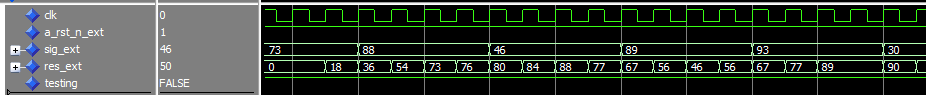
\includegraphics[width=1\textwidth]{img/Chapter4/LI_Static.png}
    \caption{Linear Interpolator First Test}
    \label{fig:LIStaticTest}
\end{figure}

In this test is possible to see that when a new signals arrives, the first of the four output signals is provided after two clock cycles. This delay is caused by the input registers and the output register that are between the input and the output of the network. 

\subsection{Linear Interpolator Dynamic Test}

As last step, a python script named \textit{TB\_Generation.py} has been created, that produces a test bench with a number of \textbf{dynamically generated stimuli}. This script takes in input as optional parameters the number of stimuli that have to generate, and the seed used for the generation (in order to have repeatable experiments).

\begin{figure}[H]
    \centering
    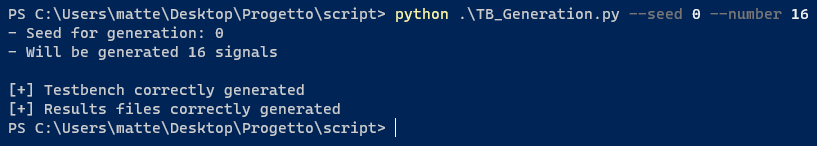
\includegraphics[width=1\textwidth]{img/Chapter4/script1.png}
    \caption{Script for Test bench Generation}
    \label{fig:Script1}
\end{figure}

The script generates three different files:

\begin{itemize}
    \item \textit{LinearInterpolator\_tb.vhd}, is generated the test bench.
    \item \textit{ExpectedResults.txt}, contains the list of the results that the circuit have to produce. It is used by a second script described below.
    \item \textit{TabulatedResults.txt}, contains the same results of previous file, but in a tabulated form, useful for an eventual visual analysis.
\end{itemize}

\begin{figure}[H]
    \centering
    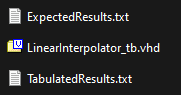
\includegraphics[width=0.4\textwidth]{img/Chapter4/GeneratedFiles.png}
    \caption{Generated Files}
    \label{fig:GenFiles}
\end{figure}

\newpage

Below there is an example of stimuli dinamically generated:

\begin{figure}[H]
    \centering
    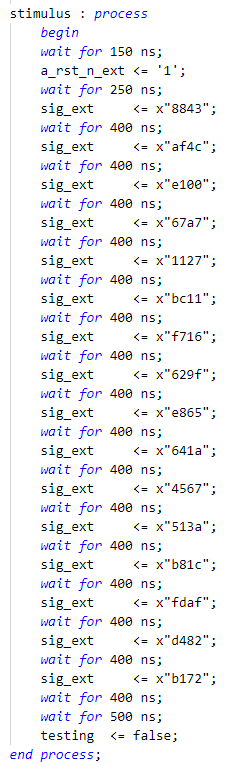
\includegraphics[width=0.4\textwidth]{img/Chapter4/GeneratedStimuli.png}
    \caption{Generated Stimuli}
    \label{fig:GenStimuli}
\end{figure}

\newpage

Instead, below there is an example of \textit{TabulatedResults.txt}:

\begin{figure}[H]
    \centering
    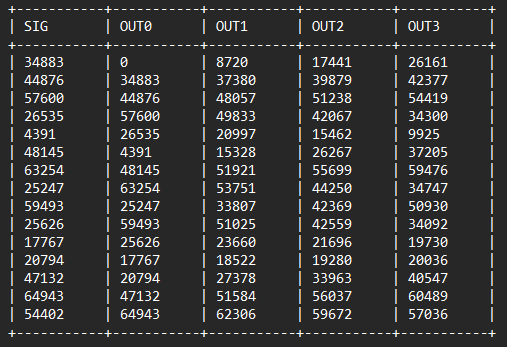
\includegraphics[width=0.6\textwidth]{img/Chapter4/ExpectedTabular.png}
    \caption{Expected Results in tabular form}
    \label{fig:ExpectedRes}
\end{figure}

The purpose of this system is to be able to test the circuit automatically and with a very large number of input signals.

For this purpose it is necessary to export from ModelSim the results obtained as output signals in a list.lst file, and run a second script (\textit{Results\_validator.py}) that compares the file exported from ModelSim with the results computed by the first script.

\begin{figure}[H]
    \centering
    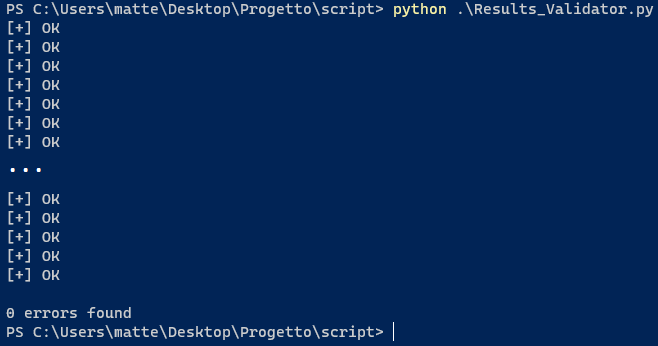
\includegraphics[width=0.6\textwidth]{img/Chapter4/Validator.png}
    \caption{Script for Results Validation}
    \label{fig:Script2}
\end{figure}

If the script finds errors, these will be notified as shown in the figure below:

\begin{figure}[H]
    \centering
    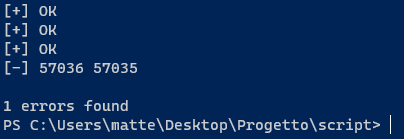
\includegraphics[width=0.6\textwidth]{img/Chapter4/Validator2.png}
    \caption{Example of wrong result}
    \label{fig:Script3}
\end{figure}